\chapter{Inégalité et fonction (rappel et compléments)}

\minitoc

Dans ce chapitre, sont rassemblés des rappels ou compléments sur les inégalités ainsi que des fondamentaux sur les fonctions de variable réelle à valeurs réelles (sans preuve ni évocation de continuité).

\section{Inégalité}

\subsection{Relation d'ordre sur \(\R\)}

\begin{defi}
	On dit que la relation \(\leq\) est une relation d'équivalence sur \(\R\) car elle vérifie les propriétés suivantes :
	\begin{enumerate}
		\item Pour tout réel x, on a : \(x \leq x \). \hfill (réfléxivité)
		\item Pour tout couple de réels \(\paren{x,y}\) tel que \( x \leq y  \) et \(y \leq x\), on a :\( y = x  \) \hfill (antisymétrie)
		\item Pour tout triplet de réels \(\paren{x,y,z}\) tel que \(x \leq y  \) et \( y \leq z  \), on a : \( x \leq z  \) \hfill (transitivité)
	\end{enumerate}
\end{defi}

\begin{prop}[Compatibilité avec les opérations]
	Soit \(x,y,z,t\) et \(a\) des réels.
	\begin{enumerate}
		\item Si \(x\leq y\) et \(z\leq t\) alors \(x+z\leq y +t \)
		\item Si \(x\leq y \) et \( 0 \leq a\) alors \(a x \leq a y\)
		\item Si \(x\leq y \) et \( a \leq 0\) alors \(a y \leq a x\)
		\item Si \( 0 \leq x \leq y \) et \( 0\leq z \leq t \) alors \( 0 \leq xz \leq y t \)
	\end{enumerate}
\end{prop}

\begin{nota}[Intervalles de \(\R\)]
	Les partie \(I\) de \(\R\) pouvant s’écrire sous l’une des formes suivantes sont dites intervalles de \(\R\) :
	\begin{itemize}
		\item \(I = \emptyset\) \\
		\item \(I = \accol{x \in \R\tq a \leq x \leq b} \underset{\mathrm{notation}}{=} \intervii{a}{b}\) avec \(\paren{a,b} \in \R^2 \) et \(a\leq b \) \\
		\item \(I = \accol{x \in \R\tq a \leq x < b} \underset{\mathrm{notation}}{=} \intervie{a}{b}\) avec \(\paren{a,b} \in \R\times \paren{\R \union \accol{\pinf}} \) et \(a < b\) \\
		\item \(I = \accol{x \in \R\tq a < x \leq b} \underset{\mathrm{notation}}{=} \intervei{a}{b}\) avec \(\paren{a,b} \in \paren{\R \union \accol{\minf}}\times \R \) et \(a < b\) \\
		\item \(I = \accol{x \in \R\tq a < x \leq b} \underset{\mathrm{notation}}{=} \intervee{a}{b}\) avec \(\paren{a,b} \in \paren{\R \union \accol{\minf}}\times  \paren{\R \union \accol{\pinf}} \) et \(a < b\) \\

	\end{itemize}
\end{nota}

\begin{prop}
	\begin{enumerate}
		\item Passage à l'inverse dans une inégalité
		      \[\quantifs{\forall x \in \Rps ; \forall y \in \Rps} x\leq y \iff \frac{1}{y} \leq \frac{1}{x}\]
		      \[\quantifs{\forall x \in \Rms ; \forall y \in \Rms} x\leq y \iff \frac{1}{y} \leq \frac{1}{x}\] \\
		\item Passage au carré dans une inégalité
		      \[\quantifs{\forall x \in \Rps ; \forall y \in \Rps} x\leq y \iff x^2 \leq y^2\]
		      \[\quantifs{\forall x \in \Rms ; \forall y \in \Rms} x\leq y \iff y^2 \leq x^2\] \\
		\item Passage à la racine carrée dans une inégalité
		      \[\quantifs{\forall x \in \Rp ; \forall y \in \Rp} x\leq y \iff \sqrt{x}\leq \sqrt{y}\] \\
		\item Passage à l’exponentielle ou au logarithme népérien dans une inégalité
		      \[\quantifs{\forall x \in \R ; \forall y \in \R} x\leq y \iff \e{x}\leq \e{y}\]
		      \[\quantifs{\forall x \in \Rps ; \forall y \in \Rps} x\leq y \iff \ln{x}\leq \ln{y}\] \\
	\end{enumerate}
\end{prop}

\begin{exoex}
	Montrer \(\quantifs{\forall x \in \intervii{0}{1}} x(1-x) \leq \frac{1}{4}\).
\end{exoex}

\begin{corr}[2 Méthode]
	Soit \(x \in \intervii{0}{1} \)
	\begin{enumerate}
		\item Raisonnement par équivalence
		      \[\begin{aligned}
				      x(1-x) \leq \frac{1}{4} & \iff 0 \leq \frac{1}{4}-x(1-x)     \\
				                              & \iff 0\leq x^2 -x +  \frac{1}{4}   \\
				                              & \iff 0\leq\paren{x- \frac{1}{2}}^2
			      \end{aligned}
		      \]
		      Ceci étant vrai \(\quantifs{\forall x\in \intervii{0}{1}}\) car \(\Delta = 0\) et \(x_0 =  \frac{1}{2}\), on conclut \(\quantifs{\forall x \in \intervii{0}{1}} x(1-x) \leq \frac{1}{4}\).\\
		\item étude de la fonction \(\fonction{f}{\intervii{0}{1}}{\R}{x}{\frac{1}{4}-x(1-x)}\)\\
	\end{enumerate}
\end{corr}


\begin{exoex}
    ~\\
	Montrer \(\quantifs{\forall x \in \Rps} x+\frac{1}{x}\geq 2\).
\end{exoex}

\begin{corr}
	Soit \(x \in \Rps \)

	\[\begin{aligned}
			x+\frac{1}{x}\geq 2 & \iff \frac{x^2+1}{x}\geq 2 \\
			                    & \iff x^2-2x+1\geq    0     \\
			                    & \iff (x-1)^2 \geq 0
		\end{aligned}
	\]
	Ceci étant vrai \(\quantifs{\forall x\in \Rps}\) on conclut \(\quantifs{\forall x \in \Rps} x+\frac{1}{x}\geq 2\).
\end{corr}

\begin{exoex}
    ~\\
	Encadrer \(\frac{2x^2-x+1}{x^2+\sqrt{x+2}+3}\) pour \(x \in \intervii{-1}{1}\).
\end{exoex}

\begin{corr}
	Soit \(x \in \intervii{-1}{1} \)
	\begin{enumerate}
		\item \underline{numérateur} :
		      \[\begin{aligned}
				      -1 \leq x\leq 1 & \iff 0 \leq x^2 \leq 1      \\
				                      & \iff 0 \leq 2x^2 \leq 2     \\
				                      & \iff 0 \leq 2x^2-x+1 \leq 4
			      \end{aligned}
		      \]

		\item \underline{denominateur} : \[\begin{aligned}
				      -1 \leq x\leq 1 & \iff 0 \leq x^2 \leq 1                                                      \\
				                      & \iff 4 \leq x^2 +\sqrt{x+2}+3 \leq 4+\sqrt{3}                               \\
				                      & \iff \frac{1}{4+\sqrt{3}} \leq \frac{1}{x^2 +\sqrt{x+2}+3 }\leq \frac{1}{4} \\
			      \end{aligned}
		      \]
	\end{enumerate}
	Ainsi par produit des deux inégalités on as \(0\leq\frac{2x^2-x+1}{x^2+\sqrt{x+2}+3}\leq1\) pour \(x \in \intervii{-1}{1}\).
\end{corr}

\begin{exoex}
    ~\\
	Encadrer \(\frac{x-y^2+3}{x^2+y^2-y}\) pour \(\forall \paren{x,y} \in \intervii{1}{2}^2\).
\end{exoex}

\begin{corr}
	Soit \(x \in \intervii{-1}{1} \)
	\begin{enumerate}
		\item \underline{numérateur} :
		      \[\begin{aligned}
				      1-4+3\leq x-y^2+3 \leq 2-1+4 & \iff 0 \leq x-y^2+3 \leq 5
			      \end{aligned}
		      \]

		\item \underline{denominateur} : \[\begin{aligned}
				      0 \leq y-1\leq 1 & \iff 0 \leq y^2-y \leq y                        \\
				                       & \iff 0 \leq y^2-y \leq 2                        \\
				                       & \iff 1 \leq x^2+y^2-y\leq 6                     \\
				                       & \iff \frac{1}{6} \leq \frac{1}{x^2+y^2-y}\leq 1 \\
			      \end{aligned}
		      \]
	\end{enumerate}
	Ainsi par produit des deux inégalités on as \(0\leq \frac{x-y^2+3}{x^2+y^2-y} \leq 5\) pour \(\forall \paren{x,y} \in \intervii{1}{2}^2\).
\end{corr}

\begin{defi}[Parties majorées, majorants, maximum]
	Une partie \(A\) de \(\R\) est dite majorée s’il existe un réel \(M\) tel que, pour tout réel \(x\) de \(A\), on a : \(x \leq M\). \\
	Un tel réel \(M\) est alors dit :
	\begin{itemize}
		\item majorant de \(A\) dans le cas général. \\
		\item maximum de \(A\) dans le cas particulier où \(M\) appartient à \(A\).\\
	\end{itemize}

\end{defi}

\begin{defi}[Parties minorées, minorants, minimum]
	Une partie \(A\) de \(\R\) est dite minorée s’il existe un réel \(m\) tel que, pour tout réel \(x\) de \(A\), on a : \(m\leq x\). \\
	Un tel réel \(m\) est alors dit :
	\begin{itemize}
		\item minorant  de \(A\) dans le cas général. \\
		\item minimum  de \(A\) dans le cas particulier où \(m\) appartient à \(A\).\\
	\end{itemize}

\end{defi}

\begin{exoex}
    ~\\
	Que dire de \(B = \accol{\frac{n}{n^2+1} \tq n \in \N}\) ?
\end{exoex}

\begin{corr}
	\begin{itemize}

		\item \(B\) est minorée car \( \quantifs{\forall n \in \N} 0 \leq \frac{n}{n^2+1} \) par ailleurs \(0 \in B\) donc \(0\) est un minimum. \\
		\item \(B\) est majorée par \(\frac{1}{2}\). En effent en notant \(U_n = \frac{n}{n^2+1}\), On voit que \((U_n)\) est strictement décroissante
	\end{itemize}
\end{corr}

\begin{exoex}
        ~\\
	Que dire de \(C = \accol{\frac{\e{x}}{x} \tq x \in \Rps}\) ?
\end{exoex}

\begin{corr}
	\begin{itemize}

		\item \(C\) est minorée car \( \quantifs{\forall x \in \Rps} 0 \leq \frac{\e{x}}{x} \) donc \(0\) est un minorant mais pas un minimum  \\
		\item Supposons que \(C\) est majorée alors \(\quantifs{\exists M \in \R,\forall c \in C} c\leq M \) ainsi \(\quantifs{\forall x \in \Rps} \frac{\e{x}}{x} \leq M \) donc par passage à la limite en \(\pinf\) on trouve \(\pinf \leq M\) ce qui est absurde donc \(C\) n'est pas majorée.
	\end{itemize}
\end{corr}

\begin{defi}[Parties bornées]
	Une partie \(A\) de \(\R\) est dite bornée si elle est majorée et minorée autrement dit s’il existe deux réels \(m\) et \(M\) tel que, pour tout réel \(x\) de \(A\), on a : \(m\leq x \leq M\).
\end{defi}

\section{Valeur absolue d'un réel}
\begin{defi}
	Pour tout \(x\) réel, la valeur absolue de \(x\), notée \(\abs{x}\), est définie par : \(\abs{x} = \begin{cases}
		-x & \text{si }  x < 0   \\
		x  & \text{si }  x\geq 0 \\
	\end{cases}\)
\end{defi}

\begin{prop}
	\begin{enumerate}
		\item Pour tout \(x\) réel, on a : \(0\leq\abs{x}\) et \(x\leq\abs{x}\)
		\item Pour tout couple\((x,y)\) de réels, on a : \(\abs{xy} = \abs{x}\abs{y}\)
		\item Pour tout couple \((x,y)\) de réels tel que \(y\) est non nul, on a: \(\abs{\frac{x}{y}} = \frac{\abs{x}}{\abs{y}}\)
	\end{enumerate}
\end{prop}

\begin{defprop}[Deux inéquations élémentaires]
	Pour tout réel \(x\) et tout \underline{réel positif} \(\alpha\), on a:
	\begin{enumerate}
		\item \(\abs{x}\leq \alpha \iff -\alpha \leq x \leq \alpha \iff x \in \intervii{-\alpha}{\alpha}\)
		\item \(\abs{x}\geq \alpha \iff x \leq -\alpha\text{ ou } \alpha \leq x \iff x \in \intervei{\pinf}{-\alpha}\union\intervie{\alpha}{\pinf}\)
	\end{enumerate}
\end{defprop}

\begin{defprop}[Interprétation sur la droite des réels]
	Soit \(a\) un réel et \(b\) un \underline{réel positif}. \\
	L’ensemble des réels \(x\) vérifiant \(\abs{x-a}\leq b\) (resp. \(\abs{ x-a}\geq b \)) est l’ensemble des points de la droite des
	réels situés à une distance du point \(a\) inférieure ou égale (resp. supérieure ou égale) à \(b\).
\end{defprop}

\begin{prop}[Inégalité triangulaire]
	Pour tout couple \((x,y)\) de réels, on a :
	\[\abs{x+y}\leq \abs{x}+\abs{y}\]
\end{prop}

\begin{dem} [inégalité triangulaire]
	Soit \((x,y) \in \R^2\)
	\begin{align*}
		\abs{x+y}\leq \abs{x}+\abs{y} & \iff \abs{x+y}^2\leq (\abs{x}+\abs{y})^2      \\
		                              & \iff x^2+2xy+y^2 \leq x^2+y^2+2\abs{x}\abs{y} \\
		                              & \iff xy\leq \abs{xy}
	\end{align*}
	Ce qui est vrai donc l'inégalité est bien démontrer
\end{dem}

\begin{exoex}   
     ~\\
	Encadrer \(\frac{x\cos(x)+1}{\sin(x)+3}\) pour \(x\in\intervii{-\pi}{2\pi}\)
\end{exoex}

\begin{corr}
	Soit \(x\in\intervii{-\pi}{2\pi}\)
	\begin{itemize}

		\item \underline{numérateur} : \(\abs{x\cos(x)+1}\leq \abs{x}\abs{\cos(x)}+1\leq 2\pi+1 = 2\pi+1\)
		\item \underline{dénominateur} : \(2\leq\abs{\sin(x)+3}\leq 4\)

	\end{itemize}
	Ainsi par produit des deux inégalités on as :\(0\leq\frac{\abs{x\cos(x)+1}}{\abs{\sin(x)+3}}\leq \frac{2\pi+1}{2} \)\\
	donc \(-\frac{2\pi+1}{2} \leq \frac{x\cos(x)+1}{\sin(x)+3} \leq \frac{2\pi+1}{2}\) pour \(x\in\intervii{-\pi}{2\pi}\).
\end{corr}

\begin{prop}
	Soit un couple \((x,y)\) de réels.
	\[\abs{\abs{x}-\abs{y}} \leq\abs{x-y}\]
\end{prop}

\begin{dem}
	Soit \((x,y) \in \R^2\)
	\(x =(x-y)+y\) donc \(\abs{x} \underset{\mathrm{\text{inég. triang.}}}{\leq} \abs{x-y}+\abs{y}\) d'où \(\abs{x} - \abs{y} \leq \abs{x-y}\) \\
	De même, \(y =(x-y)+x\) donc \(\abs{y} \underset{\mathrm{\text{inég. triang.}}}{\leq} \abs{x-y}+\abs{x}\) d'où \( -\abs{x-y} \leq\abs{x} - \abs{y}\)\\

	ainsi on a \(-\abs{x-y} \leq\abs{x} - \abs{y} \leq \abs{x-y}\) donc \(\abs{\abs{x}-\abs{y}} \leq\abs{x-y}\).
\end{dem}

\section{Partie entière d'un réel}
\begin{prop}
	Pour tout réel \(x\),il existe un unique entier \(n\) tel que :
	\[n\leq x < n+1\]
\end{prop}
\begin{defi}
	On appelle partie entière de \(x\), notée \(\lfloor x \rfloor\), l'unique entier \(n\) vérifiant la propriété précédente.
\end{defi}

\begin{ex}
	\(\lfloor 3.14 \rfloor = 3\), \(\lfloor -2.7 \rfloor = -3\) et \(\lfloor 5 \rfloor = 5\).
\end{ex}

\section{Généralité sur les fonctions}
\begin{defi} [Fonction]
	Une fonction de variable réelle à valeurs réelles notée \(f\) est un objet mathématique qui, à tout élément \(x\) d’une partie non vide de \(\R\), associe un et un seul nombre réel noté \(f(x)\). \\
	\underline{Notation Fonctionnelle} : \[\fonction{f}{A}{\R}{x}{f(x)}\]
\end{defi}

\begin{defi}
	Soit \(f\) une fonction de variable réelle à valeurs réelles.
	\begin{enumerate}
		\item L’ensemble des réels \(x\) pour lesquels \(f(x)\) existe est appelé ensemble/domaine de définition de \(f\) et souvent noté \(D_f = \accol{x \in \R \tq f(x) \text{existe}}\)
		\item Soit \(x \in D_f\)\\
		      La valeur réelle \(f(x)\) est appelée image de \(x\) par \(f\). \\
		\item soit \( y \in \R\) \\
		      S'il existe \(x\) dans \(D_f\) tel que \(f(x) = y\) alors \(x\) est dit antécédent de \(y\) par \(f\)
	\end{enumerate}
\end{defi}

\begin{defprop}[égalité entre fonction]
	Deux fonctions \(f\) et \(g\) de variable réelle à valeurs réelles sont dites égales si les deux conditions suivantes sont réunies :
	\begin{itemize}
		\item les fonctions \(f\) et \(g\) ont le même ensemble de définition \(D\) ;
		\item pour tout \(x\) de \(D\), \(f(x) = g(x)\).
	\end{itemize}
	dans ce cas, on note \(f = g\).
\end{defprop}

\begin{exoex}
	est-ce que les fonctions \(f\) et \(g\) définies par :
	\[f: x\mapsto\frac{1}{\sqrt{1+x}+1} \text{ et } g:  x\mapsto\frac{\sqrt{1+x}-1}{x}\]
	Sont égales ?
\end{exoex}
\begin{corr}
	Tout d'abord \(\quantifs{\forall x \in D_f\inter D_g} f(x) = g(x)\) car :
	\begin{align*} g(x) & = \frac{\sqrt{1+x}-1}{x}                                                 \\
                    & = \frac{\paren{\sqrt{1+x}-1}\paren{\sqrt{1+x}+1}}{x\paren{\sqrt{1+x}+1}} \\
                    & = \frac{1+x-1}{x\paren{\sqrt{1+x}+1}}                                    \\
                    & = \frac{x}{x\paren{\sqrt{1+x}+1}}                                        \\
                    & = \frac{1}{\sqrt{1+x}+1} = f(x)
	\end{align*}
	Donc \(f = g\) sur \(D_f\inter D_g\) mais
	\(D_f = \intervei{-1}{\pinf}\) or \(D_g = \intervie{-1}{\pinf}\pd\accol{0}\) donc \(D_f \neq D_g\) donc \(f \neq g\).
\end{corr}

\begin{defi}[représentation graphique d'une fonction]
	Dans le plan muni d’un repère orthonormé \((O, \vec{i}, \vec{j})\), l’ensemble de points \(\mathcal{C}_f\) défini par
	\[
		\mathcal{C}_f = \accol{ M(x; f(x)) \tq x \in D_f }
	\]
	est appelé représentation graphique de \(f\) (ou courbe représentative de \(f\)).
\end{defi}

\begin{defi}[Parité,imparité et périodicité d'une fonction]
	\begin{itemize}
		\item Une fonction \(f\) est dite paire si, pour tout \(x\) de son domaine de définition, on a : \(f(-x) = f(x)\).
		\item Une fonction \(f\) est dite impaire si, pour tout \(x\) de son domaine de définition, on a : \(f(-x) = -f(x)\).
		\item Une fonction \(f\) est dite périodique de période \(T\) si, pour tout \(x\) de son domaine de définition, on a : \(f(x+T) = f(x)\).
	\end{itemize}
\end{defi}
\begin{exo}
	Montrer que toute fonction de \(\R\) peut s'écrire de manière unique comme la somme d'une fonction paire et d'une fonction impaire.
\end{exo}

\begin{corr}[Analyse-synthèse]
	Soit \(f : \R \mapsto \R \) une fonction quelqu'onque
	\begin{itemize}
		\item \underline{Analyse} :  Supposons qu'il existe \(\begin{cases}
			      p:\R \mapsto \R \text{ paire} \\
			      i:\R \mapsto \R \text{ impaire}
		      \end{cases}\) telles que \(f = p + i\) \\
		      Ainsi \(\forall x \in \R \begin{cases}
			      f(x) = p(x) + i(x) \hfill (1)                  \\
			      f(-x) = p(-x) + i(-x) = p(x) - i(x) \hfill (2) \\
		      \end{cases}\) \\
		      \begin{itemize}
			      \item\(\frac{1}{2}\paren{\text{(1)+(2)}}\) donne \(p:x\mapsto \frac{f(x)+f(-x)}{2}\) \\
			      \item \(\frac{1}{2}\paren{\text{(1)-(2)}}\) donne \(i:x\mapsto \frac{f(x)-f(-x)}{2}\) \\
		      \end{itemize}
		\item \underline{Synthèse} : vérifions que le seul couple trouvé convient :
		      \begin{itemize}
			      \item \(\forall x \in \R, f(x) = p(x)+i(x)\)\\
			      \item \(p(-x) = p(x) \text{ et } i(-x) = -i(x)\)\\
		      \end{itemize}
	\end{itemize}
	Ainsi \(f\) s'écrit de manière unique comme la somme d'une fonction paire et impaire
\end{corr}

\begin{defi} [opération et composition]
	Soit \(f\) et \(g\) deux fonctions de variable réelle à valeurs réelles de domaines de définition \(D_f\) et \(D_g\).
	\begin{itemize}
		\item La somme de \(f\) et \(g\) est la fonction, notée \(f + g\), définie par \(f + g : x \mapsto f(x) + g(x)\). \\
		      Son domaine de définition \(D_{f+g}\) vérifie : \(D_{f+g} = D_f \inter D_g\).
		\item  La multiplication de \(f\) par le réel \(\alpha\) est la fonction, notée \(\alpha f\), définie par \(\alpha f : x \mapsto \alpha f(x)\). \\
		      Son domaine de définition \(D_{\alpha f}\) vérifie : \(D_{\alpha f} = D_f\) si \(\alpha \neq 0\).
		\item Le produit de \(f\) et \(g\) est la fonction, notée \(f g\), définie par \(f g : x \mapsto f(x)g(x)\). \\
		      Son domaine de définition \(D_{fg}\) vérifie : \(D_{fg} = D_f \inter D_g\).
		\item Le quotient de \(f\) par \(g\) est la fonction , notée \(frac{f}{g}\), définie par \(frac{f}{g} : x \mapsto \frac{f(x)}{g(x)}\). \\
		      Son domaine de définition \(D_{frac{f}{g}}\) vérifie : \(D_{frac{f}{g}} = D_f \inter \accol{x \in D_g | g(x) \neq 0}\).
		\item La composée de \(g\) et \(f\) est la fonction, notée \(g \circ f\), définie par \(g \circ f : x \mapsto g(f(x))\). \\
		      Son domaine de définition \(D_{g \circ f}\) vérifie : \(D_{g \circ f} = \accol{x \in D_f | f(x) \in D_g}\).
	\end{itemize}
\end{defi}

\begin{exoex}
	Domaine de définition de : \(\fonction{f}{D_f}{\R}{x}{\sqrt{x-\frac{1}{x}}} \)
\end{exoex}

\begin{corr}
	Soit \(x \in D_f\) alors \(x-\frac{1}{x} \geq 0 \iff x\neq 0\) et \(\frac{x^2-1}{x} = \frac{(x-1)(x+1)}{x} \geq 0\)\\
	% Assurez-vous d'avoir \usepackage{tkz-tab} dans le préambule
	\begin{tikzpicture}
		\tkzTabInit{$x$/1,$(x-1)(x+1)$/1,$x$/1,$f$/1}{$-\infty$,$-1$,$0$,$1$,$+\infty$}
		\tkzTabLine{,+,0,-,t,-,0,+,}
		\tkzTabLine{,-,t,-,0,+,t,+,}
		\tkzTabLine{,-,0,+,d,-,0,+}


	\end{tikzpicture}\\
	ainsi on voit bien que \(D_f = \intervie{-1}{0}\union\intervie{1}{\pinf}\)
\end{corr}

\section{Fonction et relation d'ordre}
\begin{defi}[Monotonie]
	Soit \(f\) une fonction de variable réelle à valeurs réelles et \(D\) une partie de son domaine de définition \(D_f\).
	\begin{enumerate}
		\item \(f\) est dite \textbf{croissante} sur \(D\) si, pour tout \((x, y) \in D^2\) tel que \(x \leq y\), on a \(f(x) \leq f(y)\).
		\item \(f\) est dite \textbf{décroissante} sur \(D\) si, pour tout \((x, y) \in D^2\) tel que \(x \leq y\), on a \(f(x) \geq f(y)\).
		\item \(f\) est dite \textbf{strictement croissante} sur \(D\) si, pour tout \((x, y) \in D^2\) tel que \(x < y\), on a \(f(x) < f(y)\).
		\item \(f\) est dite \textbf{strictement décroissante} sur \(D\) si, pour tout \((x, y) \in D^2\) tel que \(x < y\), on a \(f(x) > f(y)\).
	\end{enumerate}
	\textbf{Remarque :} \(f\) est dite \textbf{monotone} (resp. \textbf{strictement monotone}) sur \(D\) si elle est croissante ou décroissante (resp. strictement croissante ou strictement décroissante) sur \(D\).
\end{defi}

\begin{rem}[Application de la définition]
	Sous réserve que cela ait du sens :
	\begin{itemize}
		\item La somme de deux fonctions croissantes(resp. décroissantes) est croissante(resp. décroissante).
		\item La composée de deux fonctions croissantes(resp. décroissantes) est croissante(resp. décroissante).
		\item La composée d'une fonction croissante et d'une fonction décroissante est décroissante
		\item Le produit de deux fonctions \underline{positives} croissantes (resp. décroissantes) est croissante(resp. décroissante).
	\end{itemize}
\end{rem}


\begin{defi}
	Soit \(f\) une fonction de variable réelle à valeurs réelles de domaine de définition \(D_f\). \\
	Soit \(D\) une partie non vide de \(D_f\).
	\begin{enumerate}
		\item \(f\) est dite \textbf{majorée} sur \(D\) si l'ensemble \(\accol{f(x) \tq x \in D}\) est majoré, c'est-à-dire s'il existe un réel \(M\) tel que, pour tout réel \(x\) de \(D\), on a : \(f(x) \leq M\).\\
		      Un tel réel \(M\) est alors dit :
		      \begin{itemize}
			      \item \textbf{majorant} de \(f\) sur \(D\) dans le cas général.
			      \item \textbf{maximum} de \(f\) sur \(D\) dans le cas particulier où il existe \(x_0\) dans \(D\) tel que \(M = f(x_0)\).
		      \end{itemize}
		\item \(f\) est dite \textbf{minoriée} sur \(D\) si l'ensemble \(\accol{f(x) \tq x \in D}\) est minoré, c'est-à-dire s'il existe un réel \(m\) tel que, pour tout réel \(x\) de \(D\), on a : \(m \leq f(x)\).\\
		      Un tel réel \(m\) est alors dit :
		      \begin{itemize}
			      \item \textbf{minorant} de \(f\) sur \(D\) dans le cas général.
			      \item \textbf{minimum} de \(f\) sur \(D\) dans le cas particulier où il existe \(x_0\) dans \(D\) tel que \(m = f(x_0)\).
		      \end{itemize}
		\item \(f\) est dite \textbf{bornée} sur \(D\) si \(f\) est majorée et minoriée sur \(D\), c'est-à-dire s'il existe deux réels \(m\) et \(M\) tels que, pour tout réel \(x\) de \(D\), on a : \(m \leq f(x) \leq M\).\end{enumerate}
\end{defi}

\begin{prop}
	Soit \(f\) une fonction de variable réelle à valeurs réelles de domaine de définition \(D_f\). \\
	Alors \(f\) est bornée sur \(D\) si, et seulement si, la fonction \(\abs{f}\) est majorée sur \(D\).
\end{prop}
\section{Dérivation des fonctions d'une variable réelle}

\begin{defi}[dérivée en un point]
	Soit \(f\) une fonction de variable réelle à valeurs réelles de domaine de définition \(D_f\) et \(x_0\) un point de \(D_f\). \\
	\(f\) est dite dérivable en \(x_0\) si la fonction \(x\mapsto \frac{f(x)-f(x_0)}{x-x_0}\) admet une limite finie en \(x_0\). \\
	Dans ce cas, on note \(f'(x_0)\) la valeur de cette limite et on l'appelle la dérivée de \(f\) en \(x_0\). \\
	Cela reient à déterminer si la fonction \(h\mapsto \frac{f(x_0+h)-f(x_0)}{h}\) admet une limite finie en \(0\).\\
\end{defi}

\begin{defi}{fonction dérivée}
	\(f\) est dite dérivable sur \(D_f\) si elle est dérivable en tout point de \(D_f\). \\
	Dans ce cas, la fonction \(x\mapsto f'(x)\) est appelée fonction dérivée de \(f\) et notée \(f'\). \\
\end{defi}

\begin{defprop}[équation de la tangente]
	On se place dans le plan muni d’un repère orthonormé \((O, \vec{i}, \vec{j})\). \\
	Soit \(f\) une fonction de variable réelle à valeurs réelles et \(C_f\) la courbe représentative de \(f\). \\
	Soit \(x_0\) un point de \(D_f\) .\\
	Si \(f\) est dérivable en \(x_0\), alors la tangente à la courbe \(C_f\) au point \(M(x_0, f(x_0))\) est la droite d’équation :
	\[y = f'(x_0)(x-x_0) + f(x_0)\]
\end{defprop}

\begin{defprop}[opération sur les fonctions dérivable]
	Soit \(I\) et \(J\) des intervalles de \(\R\) non vide et non réduits à un point. \\
	\begin{enumerate}
		\item \underline{Combinaison linéaire} : \\
		      Soit \(f\) et \(g\) deux fonctions définies sur \(I\) et à valeurs réelles et \((\alpha, \beta)\) deux réels. \\
		      Si \(f\) et \(g\) sont dérivables sur \(I\), alors \(\alpha f + \beta g\) est dérivable sur \(I\) et sa dérivée vérifie :
		      \[\alpha f + \beta g' = \alpha f' + \beta g'\]
		\item \underline{Produit} : \\
		      Soit \(f\) et \(g\) deux fonctions définies sur \(I\) et à valeurs réelles. \\
		      Si \(f\) et \(g\) sont dérivables sur \(I\), alors \(f g\) est dérivable sur \(I\) et sa dérivée vérifie :
		      \[(f g)' =f'g+fg'\]
		      \item\underline{quotient} :\\
		      Soit \(f\) et \(g\) deux fonctions définies sur \(I\) et à valeurs réelles tel que \(g\) est non nulle sur \(I\). \\
		      Si \(f\) et \(g\) sont dérivables sur \(I\), alors \(\frac{f}{g}\) est dérivable et sa dérivée vérifie :
		      \[\paren{\frac{f}{g}}' = \frac{f'g-fg'}{g^2}\]
		\item \underline{Composition} : \\
		      Soit \(f\) une fonction définie sur \(I\) et à valeurs réelle tel que, pour tout \(x\) de \(I\), \(f(x)\) appartient à \(J\)\\
		      Soit \(g\) une fonction définie sur \(J\) et à valeurs réelles. \\
		      Si \(f\) est dérivable sur \(I\) et \(g\) dérivable sur \(J\), alors la composée \(g \circ f\) est dérivable sur \(I\) et sa dérivée vérifie :
		      \[\paren{g \circ f}' = g' \circ f \times f'\]
	\end{enumerate}
\end{defprop}

\begin{defprop}[Caractérisation des fonctions constantes ou monotones]
	Soit \(f\) une fonction définie sur un intervalle \(I\) et à valeurs réelles. \\
	\begin{enumerate}
		\item \(f\) est constante sur \(I\) si, et seulement si, pour tout \(x\) de \(I\),\(f'(x)=0\).
		\item \(f\) est croissante sur \(I\) si, et seulement si, pour tout \(x\) de \(I\), \(f'(x) \geq 0\).
		\item \(f\) est décroissante sur \(I\) si, et seulement si, pour tout \(x\) de \(I\), \(f'(x) \leq 0\).
		\item \(f\) est strictement croissante sur \(I\) si, et seulement si, les deux conditions suivante sont réunies :
		      \begin{enumerate}
			      \item pour tout \(x\) de \(I\), \(f'(x) \geq 0\) ;
			      \item il n'existe pas de réels \(a\) et \(b\) dans \(I\) avec \(a < b\) tels que pour tout \(x\) de \(\intervii{a}{b}\), on a \(f'(x) = 0\).
		      \end{enumerate}
		\item \(f\) est strictement décroissante sur \(I\) si, et seulement si, les deux conditions suivante sont réunies :
		      \begin{enumerate}
			      \item pour tout \(x\) de \(I\), \(f'(x) \leq 0\) ;
			      \item il n'existe pas de réels \(a\) et \(b\) dans \(I\) avec \(a < b\) tels que pour tout \(x\) de \(\intervii{a}{b}\), on a \(f'(x) = 0\).
		      \end{enumerate}
	\end{enumerate}
\end{defprop}

\begin{defprop}[dérivées usuelles]
    ~\\
	\begin{tabular}{|c|c|c|}

		\hline
		\textbf{Fonction}                    & \textbf{Domaine de dérivabilitée}                 & \textbf{Fonction dérivée}                                             \\
		\hline
		\(x\mapsto a\) avec \(a \in \R\)     & \(\R\)                                            & \(x\mapsto 0\)                                                        \\
		\hline
		\(x\mapsto x^n\) avec \(n \in \Ns\)  & \(\R\)                                            & \(x\mapsto nx^{n-1}\)                                                 \\
		\hline
		\(x\mapsto x^-n\) avec \(n \in \Ns\) & \(\Rs\)                                           & \(x\mapsto -nx^{-n-1}\)                                               \\
		\hline
		\(x\mapsto \sqrt{x}\)                & \(\Rps\)                                          & \(x\mapsto \frac{1}{2\sqrt{x}}\)                                      \\
		\hline
		\(x\mapsto \e{x}\)                   & \(\R\)                                            & \(x\mapsto \e{x}\)                                                    \\
		\hline
		\(x\mapsto \ln(x)\)                  & \(\Rps\)                                          & \(x\mapsto \frac{1}{x}\)                                              \\
		\hline
		\(x\mapsto \sin(x)\)                 & \(\R\)                                            & \(x\mapsto \cos(x)\)                                                  \\
		\hline
		\(x\mapsto \cos(x)\)                 & \(\R\)                                            & \(x\mapsto -\sin(x)\)                                                 \\
		\hline
		\(x\mapsto \tan(x)\)                 & \(\R\pd\accol{\frac{\pi}{2}+2k\pi \tq k \in \Z}\) & \(x\mapsto \frac{1}{\cos^2(x)} \) ou \(x\mapsto \frac{1}{\cos^2(x)}\) \\
		\hline
	\end{tabular}



\end{defprop}

\begin{exoex}
    ~\\
	Calculer\(\int_{\frac{\pi}{4}}^{\frac{\pi}{3}} \frac{\sin^3(x)}{\cos^5(x)} dx\)
\end{exoex}

\begin{corr}
	\begin{align*}
		\int_{\frac{\pi}{4}}^{\frac{\pi}{3}} \frac{\sin^3(x)}{\cos^5(x)} dx & = \int_{\frac{\pi}{4}}^{\frac{\pi}{3}} \tan^3(x) \times \frac{1}{\cos^2(x)} dx \\
		                                                                    & = \int_{\frac{\pi}{4}}^{\frac{\pi}{3}} \tan^3(x) \times \paren{\tan^2(x)+1} dx \\
		                                                                    & = \croch{\frac{1}{4}\paren{\tan^4(x) }}_{\frac{\pi}{4}}^{\frac{\pi}{3}}        \\
		                                                                    & = \frac{1}{4}\paren{\tan^4\paren{\frac{\pi}{3}} - \tan^4\paren{\frac{\pi}{4}}} \\
		                                                                    & = \frac{1}{4}\paren{\paren{\sqrt{3}}^4 - 1^4}                                  \\
		                                                                    & = 2                                                                            \\
	\end{align*}
\end{corr}

\begin{defprop}[étude pratique d'une fonction]
	Le plan d'étude d'une fonction \(f\) est en général le suivant:
	\begin{itemize}
		\item Détermination du domaine de définition de \(f\)
		\item Réduction éventuelles du domaine d'étude selon les propriétés de \(f\) (parité, périodicité, etc.)
		\item Limites aux bornes du domaine d'étude
		\item Etude de la monotonie (le plus souvent,mais pas uniquement, après calcul de la dérivée de \(f\) et détermination du signe de celle-ci )
		\item Construction du tableau de variation de \(f\)(limites aux bornes, valeurs remarquables, variations)
		\item Tracé de la courbe représentative de \(f\)
	\end{itemize}
\end{defprop}
\begin{defprop}[dérivées d'odre supériéur]
	Soit \(f\) une fonction définie sur un intervalle \(I\) et à valeurs réelles. \\
	On note
	\[f^{(0)} = f\]
	puis, pour tout entier naturel \(k\) tel que la fonction\(f^{(k)}\) existe et est déribable sur \(I\), on pose :
	\[f^{(k+1)} = \paren{f^{(k)}}'\]
	Si \(n\) est un entier naturel, tel que la fonction \(f^{(n)}\) existe alors on dit que \(f\) est \(n\)-fois dérivable sur \(I\) et que \(f^{(n)}\) est la dérivée d'ordre \(n\) (ou dérivée \(n\)-ième) de \(f\).\\

\end{defprop}
\begin{defi}[Fonction réciproque]
	Soit \(f\) une fonction définie sur un intervalle \(I\) à valeurs dans \(J\)
	Si, pour tout y de \(J\), l’équation \(y = f(x)\) admet une unique solution \(x\) dans \(I\) notée \(x = f^{-1}(y)\) alors :
	\begin{itemize}
		\item la fonction \(f\) est dite bijection de \(I\) sur \(J\)
		\item la fonction \(f^{-1}\) ainsi définie sur \(J\) et à valeurs dans \(I\), est dite bijection réciproque de \(f\).
	\end{itemize}
	\underline{Exemples}:
	\begin{itemize}
		\item \(\sqrt{}\) est une bijection de \(\Rp\) sur \(\Rp\) de bijection réciproque \(f : \Rp \to \Rp\) définie par \(f(x) = x^2\).
		\item \(\exp\) est une bijection de \(\R\) sur \(\Rps\) de bijection réciproque la fonction \(\ln\)
	\end{itemize}
\end{defi}
\begin{prop}[Propriétés de la bijection réciproque]
	Si \(f\) est une bijection de \(I\) sur \(J\) de bijection réciproque notée \(f^{-1}\) alors on a :
	\begin{enumerate}
		\item pour tout \(x\) de \(I\), \(f(f^{-1}(x)) = x\) ;
		\item pour tout \(y\) de \(J\), \(f^{-1}(f(y)) = y\).
	\end{enumerate}

\end{prop}

\begin{defprop}[représentation graphique]
	on se place dans le plan muni d’un repère orthonormé \((O, \vec{i}, \vec{j})\). \\
	Si \(f\) est une bijection de \(I\) sur \(J\) alors la courbe représentative de \(f\) et de sa bijection réciproque \(f^{-1}\) sont symétriques par rapport à la droite d’équation \(y = x\).
\end{defprop}

\begin{defprop}[dérivée de la bijection réciproque]
	Soit \(f\) une bijection de \(I\) sur \(J\)  et si \(f\) est dérivable sur \(I\) alors sa bijection réciproque \(f^{-1}\) est dérivable en tout point y de \(J\) tel que \(f'(f^{-1}(y)) \neq 0\) avec, dasn ce cas : \[(f^{-1})'(y) = \frac{1}{f'(f^{-1}(y))}\]
\end{defprop}
\begin{dem}
	Soit \(f\) une bijection de \(I\) sur \(J\), soit \(y\) in \(J\) tel que \(f'(f^{-1}(y)) \neq 0\). \\
	on sait que \(f(f^{-1}(y)) = y\) donc en appliquant la définition de la dérivée de fonction composée on a :
	\[(f(f^{-1}(y)))' = (y)' \iff f'(f^{-1}(y))\times (f^{-1}(y))' = 1 \iff (f^{-1}(y))' = \frac{1}{f'(f^{-1}(y))}\]
\end{dem}
\begin{defprop}[Trois fonction usuelles trigonométriques]
	\begin{itemize}
		\item \underline{Fonction \(\Arccos\)} : \\
		      La fonction \(\Arccos\) est la réciproque de la fonction \(\fonction{c}{\intervii{0}{\pi}}{\intervii{-1}{1}}{x}{\cos(x)}\) et est donc définie sur \(\intervii{-1}{1}\) à valeurs dans \(\intervii{0}{\pi}\) et dérivable sur \(\intervee{-1}{1}\) de dérivée: \[\arccos':x\mapsto \frac{-1}{\sqrt{1-x^2}}\]\\
		\item \underline{Fonction \(\Arcsin\)} : \\
		      La fonction \(\Arccos\) est la réciproque de la fonction \(\fonctionlambda{\intervii{-\frac{\pi}{2}}{\frac{\pi}{2}}}{\intervii{-1}{1}}{x}{\sin(x)}\) et est donc définie sur \(\intervii{-1}{1}\) à valeurs dans \(\intervii{-\frac{\pi}{2}}{\frac{\pi}{2}}\) et dérivable sur \(\intervee{-1}{1}\) de dérivée: \[\arcsin':x\mapsto \frac{1}{\sqrt{1-x^2}}\]\\
		\item \underline{Fonction \(\Arctan\)} : \\
		      La fonction \(\Arccos\) est la réciproque de la fonction \(\fonctionlambda{\intervee{-\frac{\pi}{2}}{\frac{\pi}{2}}}{\R}{x}{\tan(x)}\) et est donc définie sur \(\R\) à valeurs dans \(\intervee{-\frac{\pi}{2}}{\frac{\pi}{2}}\) et dérivable sur \(\R\) de dérivée: \[\arctan':x\mapsto \frac{1}{1+x^2}\]\\
	\end{itemize}
\end{defprop}


\begin{dem}[démonstration de la dérivée de la fonction \(\Arccos\)]
	Soit \(y\in\intervii{-1}{1}\), on note \(\fonction{c}{\intervii{0}{\pi}}{\intervii{-1}{1}}{x}{\cos(x)}\)
	\begin{align*}
		c'(c^{-1}(y)) & = -\sin(c^{-1}(y))                                                                                                \\
		              & = -\sqrt{\sin^2(c^{-1}(y))} \qquad  \text{car }c^{-1}(y)\in \intervii{0}{\pi} \text{ donc } \sin(c^{-1}(y))\geq 0 \\
		              & = -\sqrt{1-\cos^2(c^{-1}(y))}                                                                                     \\
		              & = -\sqrt{1-y^2}                                                                                                   \\
	\end{align*}
	Ainsi d'après la définition de la dérivée de la bijection réciproque on a : \(\Arccos'(y) = \frac{-1}{\sqrt{1-y^2}}\)
\end{dem}

\begin{rem}[démonstration d'une relation intéressante entre \(\Arctan(x)\) et \(\Arctan\paren{{\frac{1}{x}}}\)]
	Soit \(f:x\mapsto \Arctan{\paren{\frac{1}{x}}}\), on as \(D_f = \R\pd\accol{0}\) et \(f\) dérivable sur \(D_f\)
	\begin{align*}
		f'(x) & = \Arctan'\paren{\frac{1}{x}} \times \paren{\frac{1}{x}}'         \\
		      & = \frac{1}{1+\paren{\frac{1}{x}}^2} \times \paren{\frac{-1}{x^2}} \\
		      & = \frac{-1}{x^2+1}
	\end{align*}
	On remarque que \(\quantifs{\forall x \in \Rs}f'(x) = -\Arctan'\paren{x}\) ainsi \(\quantifs{\forall x \in \Rps}f'(x) +\Arctan'\paren{x} = 0\) donc \(\quantifs{\forall x \in \Rs}\paren{f(x)+\Arctan\paren{x}}'=0\) \\
	Ainsi il existe \(c\) un réel tel que \(\quantifs{\forall x \in \Rps}f(x) + \Arctan\paren{x} = c\)
	\begin{align*}
		\text{Pour } x = 1, f(1) + \Arctan(1) & = c \\
		f(1) + \frac{\pi}{4}                  & = c \\
		c = \frac{\pi}{2}
	\end{align*}
	Ainsi \(\quantifs{\forall x \in \Rps} \Arctan\paren{\frac{1}{x}} + \Arctan\paren{x} = \frac{\pi}{2}\) \\
	De manière analogue on trouve  \(\quantifs{\forall x \in \Rms} \Arctan\paren{\frac{1}{x}} + \Arctan\paren{x} = -\frac{\pi}{2}\) \\
\end{rem}